% =============================================================================
% PRL variant of the troposwhere manuscript (K=5).
% Reformatted from the Nature-Comp-Sci article-class version
% (preserved in main_natcomp_backup.tex) into REVTeX 4.2 / Physical Review
% Letters format: two-column reprint layout, numeric APS citations
% (apsrev4-2.bst), PRL title/abstract block.
%
% CONVERSION STATUS (pass 1 = reformat; content preserved, not yet cut to
% the PRL length limit ~3750 words / 4 pages):
%   [x] REVTeX 4.2 preamble, prl option, two-column reprint
%   [x] Numeric \cite throughout (was authoryear \citep/\citet)
%   [x] Title / author / affiliation / abstract block
%   [x] Body ported (intro + results + discussion)
%   [x] Methods kept at end (candidate for Supplemental Material / End Matter)
%   [ ] Cut to PRL length (pass 2)
%   [ ] Split heavy Methods -> Supplemental Material (pass 2)
%   [ ] Verify author affiliations (marked TODO below)
% =============================================================================
% Review layout: reprint class (compact title block -> abstract on page 1,
% no empty title page), but the body is forced to a single wide column via
% \onecolumngrid after \maketitle so that line numbers sit cleanly in the
% left margin without the two-column gutter overlap. For the final
% journal-look two-column preview, comment out the \onecolumngrid line below.
\documentclass[
    aps,
    prl,
    reprint,
    superscriptaddress,
    amsmath,amssymb,
    floatfix,
    nofootinbib
]{revtex4-2}

% ── Figures, math, typography ──────────────────────────────────────────
\usepackage{graphicx}
\usepackage{bm}
\usepackage{xcolor}
\usepackage[colorlinks=true,allcolors=blue!50!black,citecolor=blue!50!black]{hyperref}
\usepackage{xr-hyper}                             % cross-refs to Supplemental Material labels
\externaldocument[S]{supplementary}                  % reads supplementary.aux (build SM first)
\usepackage{lineno}                               % line numbers (clean in single-column preprint)
\usepackage{setspace}                             % wider line spacing for the review copy
% \linenumbers is issued after \maketitle (below) to avoid a lineno/REVTeX
% interaction that pushes the abstract onto a blank second page.

\graphicspath{{./}{figures/}{SI_figures/}{img/}}

\begin{document}

\title{A temporally-constrained latent space reveals the stochastic dynamics of convective organization}

\author{Sophie Abramian}
\affiliation{Department of Earth and Environmental Engineering, Columbia University, New York, NY, USA}

\author{Olivier Pauluis}
\affiliation{Courant Institute of Mathematical Sciences, New York University, New York, NY, USA}

\author{Pierre Gentine}
\affiliation{Department of Earth and Environmental Engineering, Columbia University, New York, NY, USA}

\date{\today}

\begin{abstract}
Atmospheric convection is stochastic: under fixed forcing, storms take different trajectories. We introduce an unsupervised framework that encodes isentropic mass-flux fields from cloud-resolving squall-line simulations into a latent space constrained by a linear operator predicting the next step. Five convective states emerge without supervision; their transitions form a Markov chain with a slow eigenmode alternating two main regimes, organized and unorganized. Residual non-Markovian memory is partly carried by cold pools, offering a stochastic alternative to multi-cloud parameterizations.
\end{abstract}

\maketitle
\onecolumngrid   % single-column body for clean line numbers (comment out for 2-column preview)
\onehalfspacing  % wider line spacing to make the review easier
\linenumbers

% ── Introduction (no heading, PRL Letter style) ────────────────────────
Discovering interpretable, low-dimensional representations of high-dimensional stochastic dynamics is a foundational challenge across the physical sciences. Deep convection in the atmosphere is a prime example. Deep convective systems---organized cloud structures larger and longer-lived than individual cells---dominate the tropical water and energy cycle \cite{houze2004mesoscale, chakraborty2023overview}; the largest, mesoscale convective systems, contribute over 50\% of tropical precipitation and a disproportionate share of extremes \cite{roca2020extreme, feng2024mesoscale, feng2023mesoscale}.

In climate models they occur below the grid scale and must be parameterized---a persistent source of uncertainty, especially under warming \cite{yang2023impact, bolot2025no}. The difficulty is that a convective system is a high-dimensional dynamical object; compressing it into a few prognostic variables without discarding what matters is hard.

Compounding this, the convective response to a \emph{fixed} large-scale forcing is not a single outcome but a broad distribution of storm evolutions \cite{abramian2025key, feng2025mesoscale, hu2020observed, fiolleau2024database}---an \emph{internal} variability intrinsic to the convection, not inherited from the environment. Capturing it requires a reduced description that is both low-dimensional and faithful to the dynamics.

Stochastic multi-cloud models \cite{khouider2006multicloud, majda2008stochastic, khouider2010stochastic} offer such a reduction, but a strongly simplified one whose states are prescribed \emph{a priori}: a lattice of sites, each in one of a few hand-chosen cloud states---clear sky, shallow, congestus, or deep---whose area fractions evolve by a Markov chain. This captures the changing cloud cover but not the vertical mass-flux profiles that in addition govern extreme precipitation \cite{MullerYukari19, singh2012upward, abramian2023extreme, wang2022convective, li2025bimodal}.

Koopman operator theory \cite{koopman1931hamiltonian, brunton2021modern} offers a principled alternative. Instead of the state $\mathbf{x}_t$ of a high-dimensional nonlinear system, one follows \emph{observables} $g(\mathbf{x})$ that recast it in new coordinates; the operator advancing them---$\mathcal{K}$, the Koopman operator, defined by $(\mathcal{K}g)(\mathbf{x}_t) = g(\mathbf{x}_{t+1})$---is linear by construction, whatever the nonlinear dynamics. The challenge is thus not to resolve the nonlinear evolution, but to find an observable that simplifies it---ideally one on which $\mathcal{K}$ acts as a simple multiplication---while retaining most of the system's information. Such an observable is generally infinite-dimensional \cite{brunton2021modern}---the long-standing obstacle. Only recently have machine-learning encoder--decoder architectures \cite{lusch2018deep, nathaniel2026generative} overcome it, learning from data the best finite-dimensional observable for a given latent dimension together with its linear operator.

We depart from existing Koopman autoencoders in two ways. First, we start from a physically reduced representation of the system, casting the flow in isentropic coordinates \cite{pauluis2013isentropic}---a thermodynamically consistent reduction that filters reversible adiabatic motions---rather than using the raw, noisy three-dimensional fields. Second, rather than enforcing \emph{deterministic} linear dynamics, we \emph{partition} the latent space into discrete states by joint clustering \cite{kaiser2014cluster, souza2024representing} and model their transitions \emph{probabilistically}. The result is a Markov chain on data-discovered states---finite-dimensional, stochastic, and shaped by the dynamics it represents. Though demonstrated on convection, the framework applies to any high-dimensional system where regime discovery and transition modeling are needed.

We analyze cloud-resolving simulations of squall lines (SAM~\cite{khairoutdinov2003}) under fixed vertical wind shear, in statistical equilibrium yet with strong internal variability. Convection is cast in isentropic coordinates: at each time the three-dimensional vertical mass flux is projected onto height $z$ and moist static energy $h$, yielding a two-dimensional diagram $M(h,z)$ that cleanly separates high-$h$ updrafts from the low-$h$ evaporative downdrafts that build cold pools~\cite{pauluis2013isentropic}. Figure~\ref{fig:simu_isentrop} shows three representative snapshots---suppressed, organized-deep, and unorganized-active convection---alongside their mass-flux diagrams; this time series of diagrams is the input to the model.

\begin{figure}[t]
    \centering
    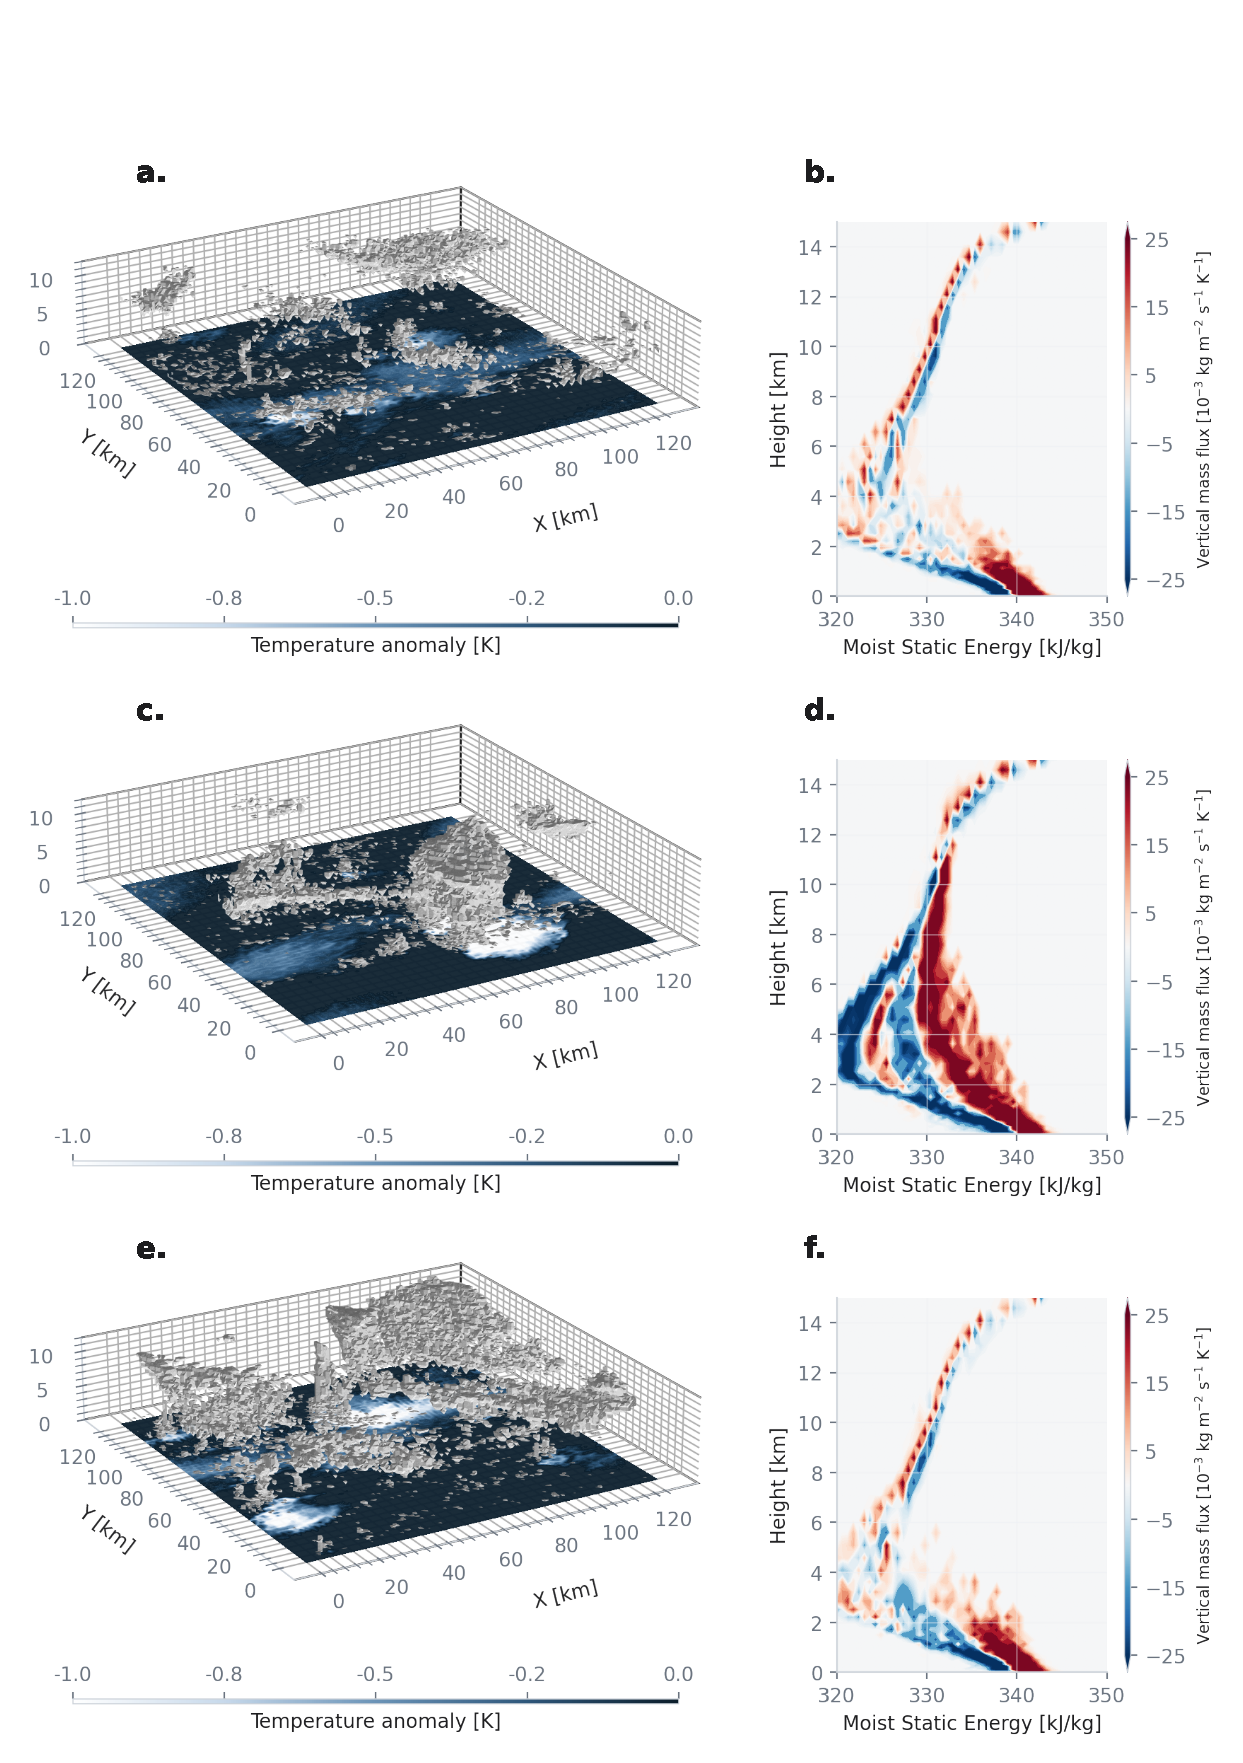
\includegraphics[width=0.62\textwidth]{fig1_snapshots.pdf}
    \caption{\textbf{Three contrasting snapshots of the simulated convective field.} \textbf{Left (a, c, e):} isovolume of non-precipitating condensate $\mathrm{QN}=0.02$~kg\,kg$^{-1}$ over the surface temperature anomaly; white patches mark cold pools. \textbf{Right (b, d, f):} the corresponding isentropic mass-flux diagram $M(h,z,t)$, red (blue) for upward (downward) transport. Rows: \textbf{(a--b)} suppressed, \textbf{(c--d)} organized deep, and \textbf{(e--f)} unorganized active convection.}
    \label{fig:simu_isentrop}
\end{figure}

Applied to these simulations, the construction asks: (i) what mass-flux states a given forcing makes accessible; (ii) whether their transitions form a Markov chain, and how organized and weakly organized pathways differ; (iii) where internal feedbacks---cold pools in particular---introduce memory beyond the discrete state. Five interpretable states emerge without supervision, and their transitions form a Markov chain with a slow ($\sim$3\,h) eigenmode alternating two regimes, organized and unorganized; two long-lived states decay more slowly than their Markov prediction, and conditioning on cold-pool intensity closes $\sim$30\% of that gap.

% ── Results ────────────────────────────────────────────────────────────
\section{Construction and physical interpretation of the latent space}

The squall-line evolution is seen through its time series of isentropic mass-flux fields $X_t$. The model compresses each field into a latent vector $\mathbf{z}_t\in\mathbb{R}^8$ and groups it into five discrete states. Specifically, an encoder maps $X_t$ to a Gaussian posterior over $\mathbf{z}_t$ (a variational autoencoder with reconstruction and Kullback--Leibler terms); a softmax head turns $\mathbf{z}_t$ into a probability vector $s_t$ over the $K=5$ states; and a row-stochastic matrix $\mathbf{T}$ propagates it one step, $s_{t+1}\approx\mathbf{T}\,s_t$. These three components are trained jointly on consecutive pairs $(X_t, X_{t+\Delta t})$, so the latent space is at once reconstructive, cluster-separable, and dynamically predictive (Fig.~\ref{fig:model}). A contrastive loss based on the structural (Dice) similarity of the mass-flux fields prevents state collapse, keeping all five states populated. Full architecture, losses, and training are given in the Supplemental Material.

\begin{figure}[!ht]
    \centering
    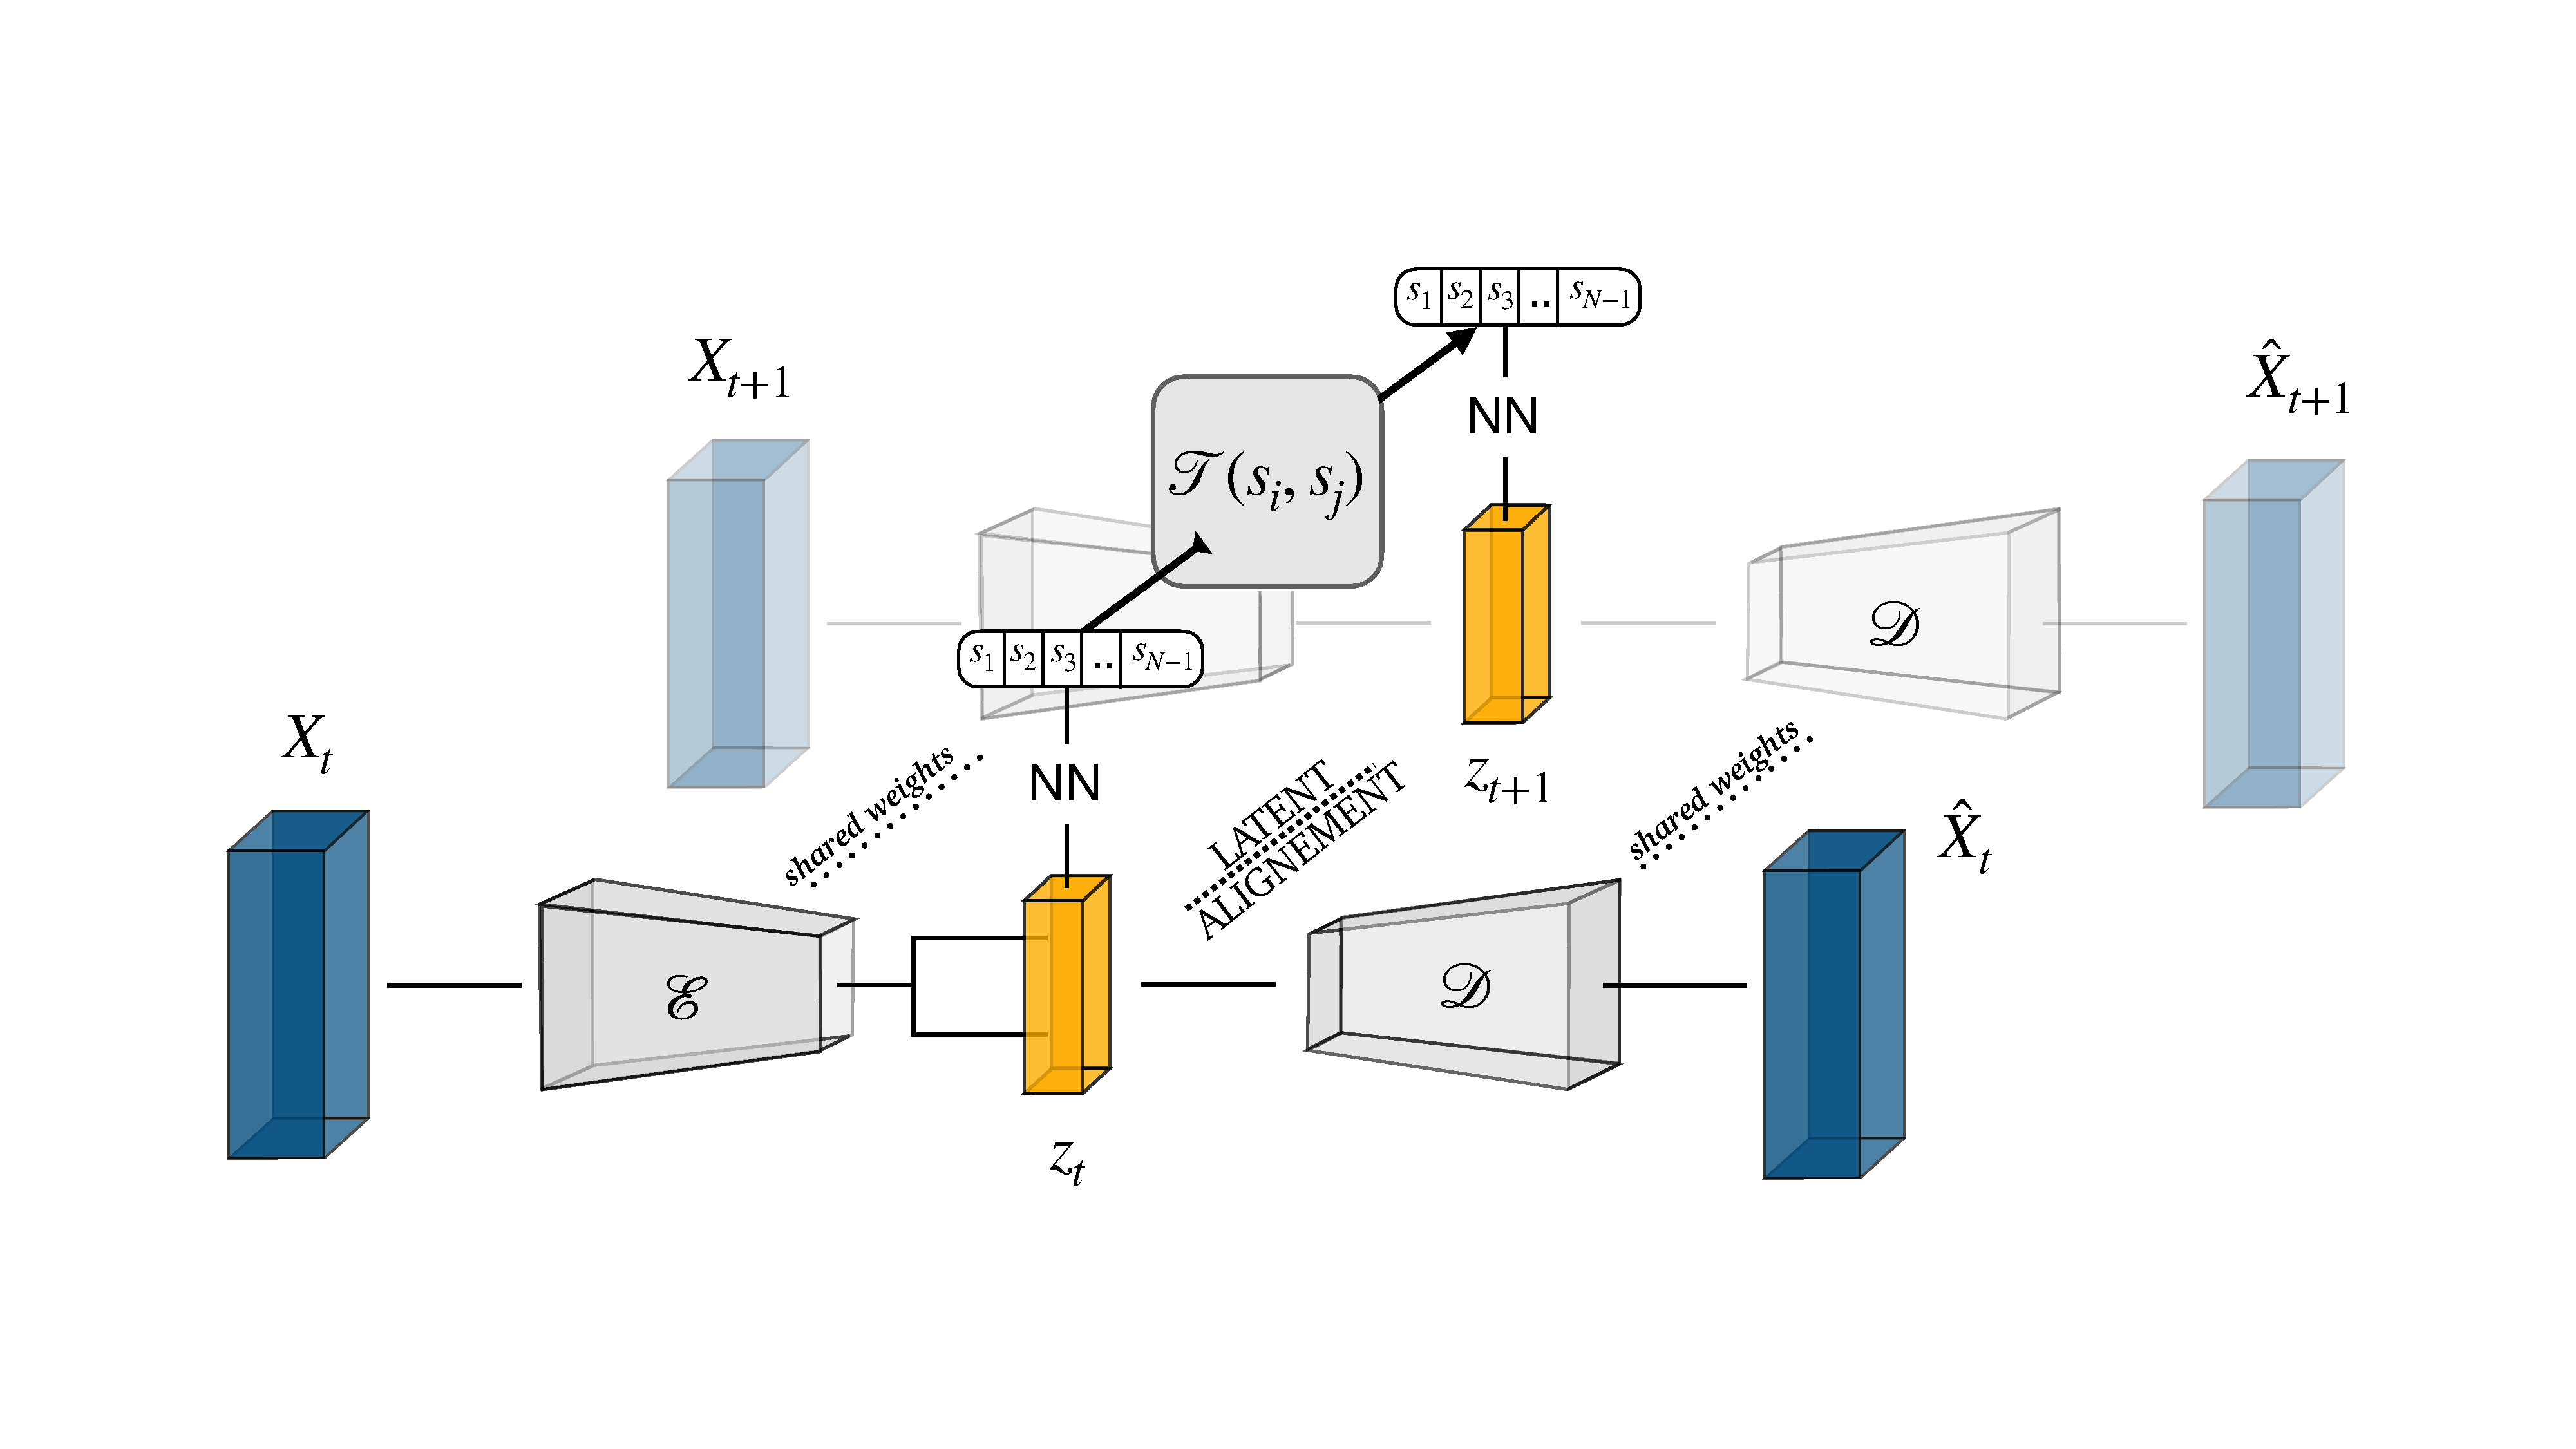
\includegraphics[width=0.78\textwidth]{model_vae_mc.pdf}
    \caption{\textbf{Model architecture.} A variational autoencoder (VAE) is coupled to a Markovian state-assignment and transition framework. An encoder maps the input to a latent representation $z_t$, reconstructed by a decoder; a small network assigns each $z_t$ a probability distribution over $K=5$ discrete states; and a linear transition operator $T$ predicts the state distribution at $t+1$ from that at $t$.}
    \label{fig:model}
\end{figure}

No physical constraint is imposed during training---the VAE is regularized only toward an isotropic Gaussian, and states are assigned without reference to intensity, organization, or any diagnostic---so whether the latent space is physically meaningful is not guaranteed. Applying PCA to $\mathbf{z}(t)$, the first two components explain $22\%$ and $17\%$ of the variance (Fig.~\ref{fig:clusters}); a three-dimensional projection (Supplemental Material, Fig.~\ref{Sfig:pca_3d}) shows that states overlapping in 2D separate along higher-order components.

\begin{figure*}[t]
    \centering
    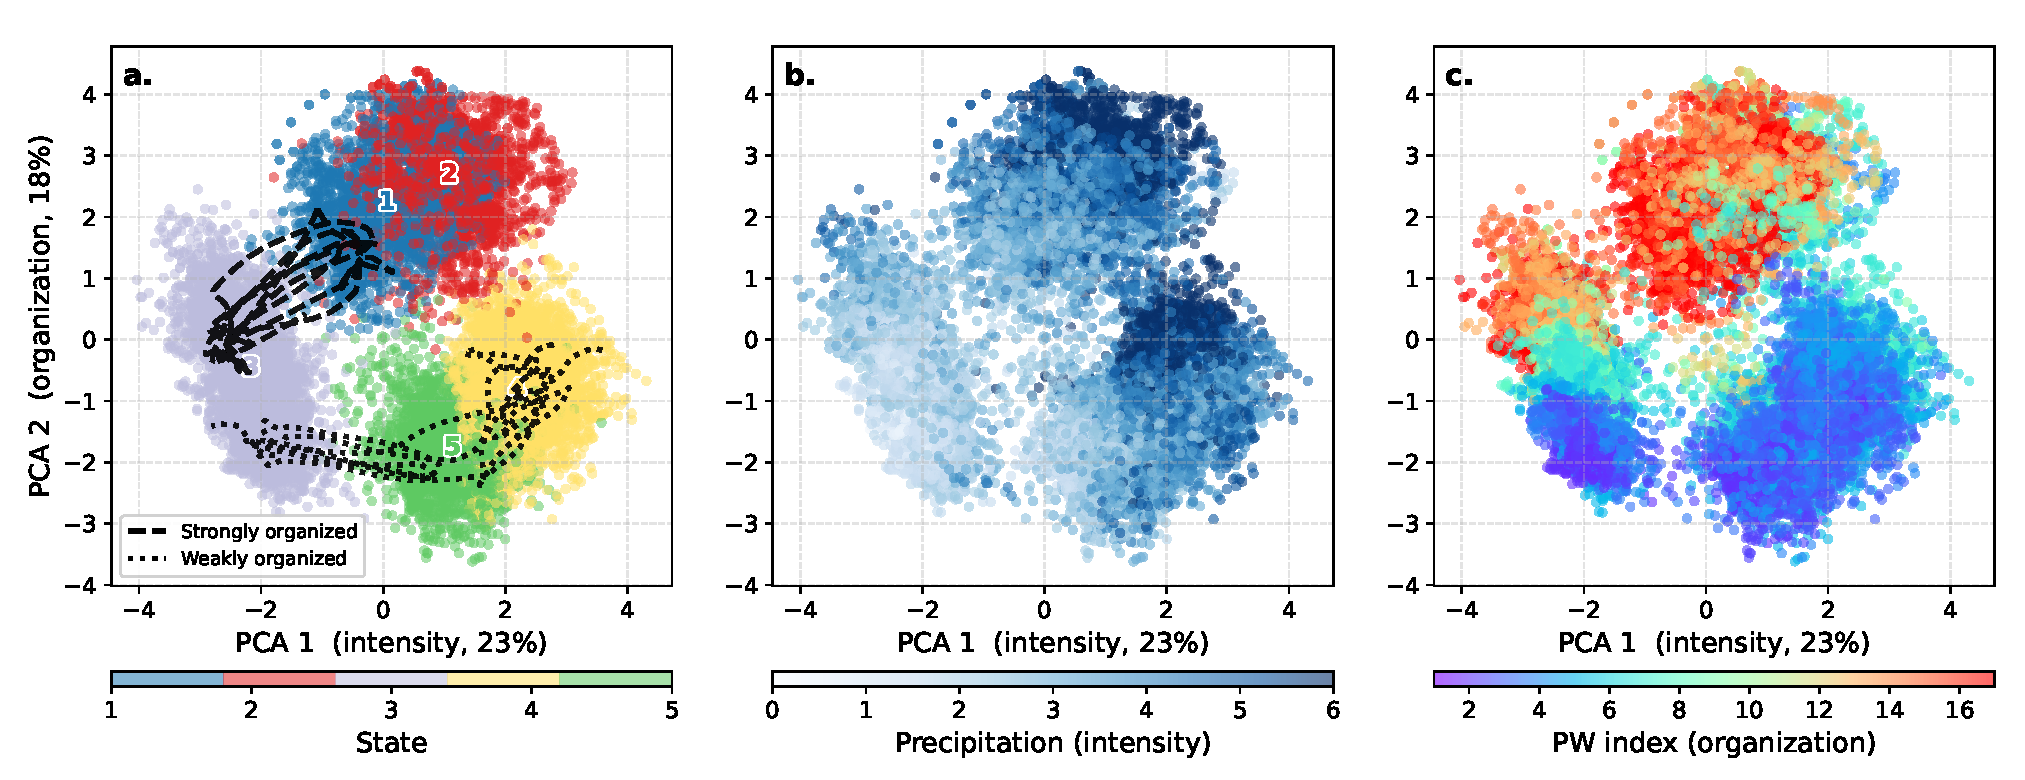
\includegraphics[width=0.98\textwidth]{fig_pca_panels.pdf}
    \caption{\textbf{Latent-space visualization and physical interpretation.} PCA projection of the latent space (each point is one time step), coloured by \textbf{(a)}~state assignment, with two example trajectories over 5~h (dashed: strongly organized; dotted: weakly organized; time series in the Supplemental Material); \textbf{(b)}~domain-mean precipitation, a proxy for convective intensity; and \textbf{(c)}~the variance of precipitable water (the PW index), a proxy for spatial organization (higher values indicate more clustered convection). The first component (PCA~1) aligns with intensity, the second (PCA~2) with organization; joint distributions of the two components against these diagnostics are given in the Supplemental Material (Fig.~\ref{Sfig:axis_var}).}
    \label{fig:clusters}
\end{figure*}

The dominant latent directions are physically interpretable (Fig.~\ref{fig:clusters}). The first principal component correlates strongly with domain-mean precipitation---convective intensity and life-cycle stage, from suppressed to vigorously precipitating. The second is nearly uncorrelated with precipitation but strongly anticorrelated with the variance of precipitable water, a proxy for spatial organization. Intensity and organization thus emerge as two largely independent axes of the learned representation.

The five states are also dynamically and thermodynamically distinct. Averaging the isentropic mass flux within each state as anomalies from the simulation-wide mean (definitions and full profiles in the Supplemental Material) shows that the organized-deep and stratiform-like states carry deep, high--moist-static-energy ascent---the stratiform-like state additionally showing a mid-level mass-flux signature suggestive of stratiform detrainment---while the active-unorganized state peaks at lower altitude and lower moist static energy, and the suppressed and shallow-congestus states carry only weak, shallow anomalies. Table~\ref{tab:state_summary} summarizes each state.

\begin{table}[t]
\centering
\begin{ruledtabular}
\begin{tabular}{c l c p{0.42\textwidth}}
State & Name & $\pi$ (\%) & Physical signature \\
\hline
1 & \emph{Organized deep}     & 12.9 & sustained deep ascent in a moist environment; reduced low-level detrainment; highest precipitable-water variance \\
2 & \emph{Stratiform-like}    & 12.2 & strongly active convection with large upper-tropospheric mass flux, consistent with a mesoscale stratiform region; highest precipitation \\
3 & \emph{Suppressed convection} & 37.0 & weak up- and down-drafts; dry background atmosphere; dominant state \\
4 & \emph{Active unorganized}     & 22.7 & active but unorganized convection, with mass flux peaking at lower altitudes than in the organized regime; drier environment \\
5 & \emph{Shallow congestus}      & 15.2 & suppressed deep convection with residual shallow convective activity; dry environment \\
\end{tabular}
\end{ruledtabular}
\caption{\textbf{Summary of the five latent convective states.} State identities are inferred from the latent-space axes of variability (Fig.~\ref{fig:clusters}) and confirmed by the per-state vertical and moist-static-energy mass-flux profiles (Supplemental Material). $\pi_i$ is the stationary probability of state~$i$ [Eq.~\eqref{eq:canon}].}
\label{tab:state_summary}
\end{table}

\section{Markov transition matrix, eigenmodes, and regimes}

The second output of the model is a Markov transition matrix $\mathbf{T}$, whose elements
\begin{equation}
T_{ij} = \mathbb{P}\left( X_{t+\Delta t} = j \mid X_t = i \right)
\end{equation}
denote the probability of transitioning from state $i$ to state $j$. The resulting transition matrix is shown in Fig.~\ref{fig:markov_matrix}.

\begin{figure*}[t]
    \centering
    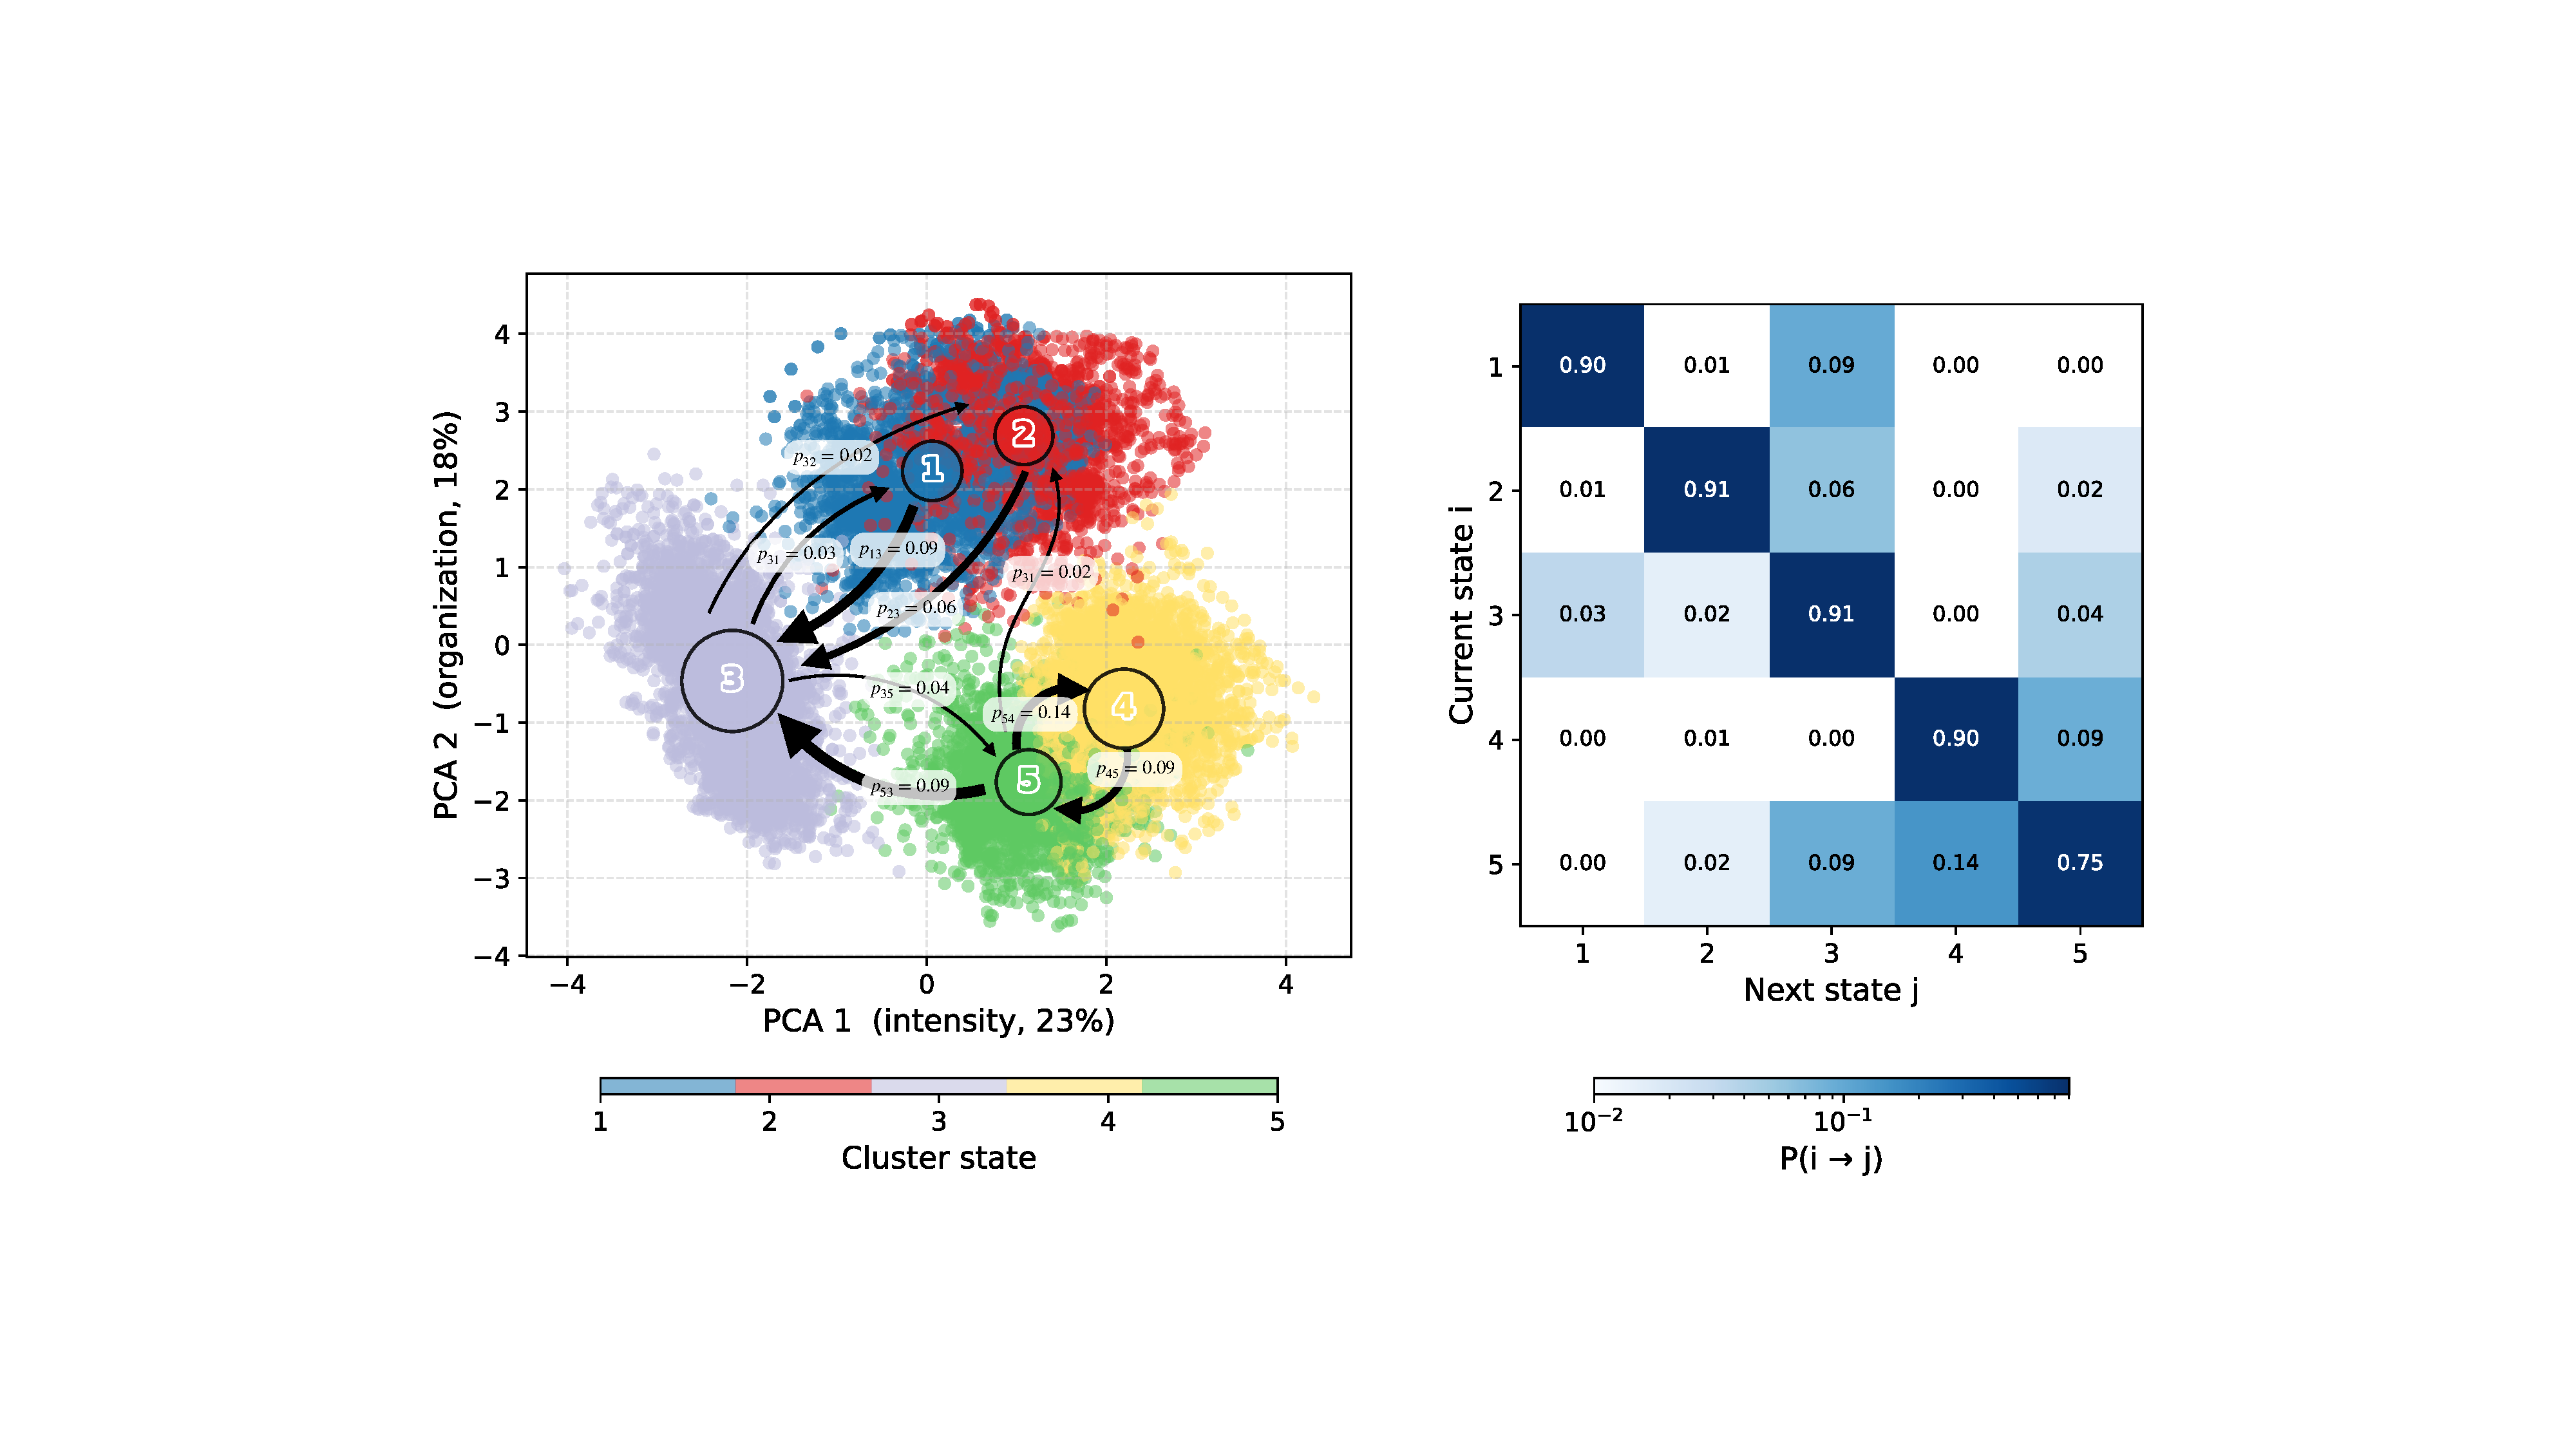
\includegraphics[width=0.92\textwidth]{fig7_markov_matrix.pdf}
    \caption{\textbf{Markov state dynamics in latent space.} \textbf{(A)} Latent space visualization with the inferred Markov chain overlaid. The size of each state node is proportional to its asymptotic (stationary) probability, and arrows indicate transition probabilities between states. \textbf{(B)} Transition matrix describing the dynamics of convection for the given shear. Two coupled blocks, separated by state~3, form the organized (states~1--2) and unorganized (states~4--5) regimes.}
    \label{fig:markov_matrix}
\end{figure*}

The matrix $\mathbf{T}$ is strongly diagonally dominated, indicating that the system tends to persist within a given state over several time steps. Moreover, the matrix is sparse, with only a limited number of preferred transitions between states, suggesting constrained pathways in state space.

To further characterize the dynamics, we perform a spectral decomposition of $\mathbf{T}$. Because $\mathbf{T}$ is stochastic, it admits a unit eigenvalue $\lambda_1=1$. The corresponding right eigenvector $\boldsymbol{\pi}$ satisfies $\mathbf{T}\boldsymbol{\pi}=\boldsymbol{\pi}$ and defines the stationary distribution of the Markov chain. We obtain
\begin{equation}
\boldsymbol{\pi} =
\begin{bmatrix}
12.9\% & 12.2\% & 37.0\% & 22.7\% & 15.2\%
\end{bmatrix}.
\label{eq:canon}
\end{equation}

The stationary distribution is dominated by state~3 ($37\%$, suppressed convection), the remaining weight spread across the four active states---all sufficiently populated to constrain the inferred transition statistics.

We next examine the subdominant eigenvalues and eigenvectors of $\mathbf{T}$. All non-stationary eigenvalues have imaginary parts at the level of numerical noise ($|\mathrm{Im}(\lambda_k)|<10^{-3}$); the spectrum is effectively real. This indicates that the dominant dynamics cannot be described as simple linear oscillations in state space.

The leading nontrivial eigenvalue of the transition matrix is $\lambda_2 \approx 0.94$, indicating a highly persistent dynamical mode. The corresponding eigenvector
\begin{equation}
\mathbf{v}_2 =
\begin{bmatrix}
-0.56 & -0.30 & -0.25 & +0.65 & +0.34
\end{bmatrix}
\end{equation}
is unit-norm (the overall sign is arbitrary). A positive $(\mathbf{v}_2)_i$ means state~$i$ is enhanced relative to $\pi_i$ in one phase of this mode and suppressed in the other; $|(\mathbf{v}_2)_i|$ sets the relative size of that deviation across states. Components of opposite sign therefore vary in anti-phase.

The components of $\mathbf{v}_2$ split the chain into two opposite-sign groups, $\{1,2\}$ ($-0.56,\,-0.30$) and $\{4,5\}$ ($+0.65,\,+0.34$); state~3 has the smallest amplitude in this mode ($-0.25$). We interpret these two groups as two convective regimes---\emph{organized} ($\{1,2\}$) and \emph{unorganized} ($\{4,5\}$)---that the chain alternates between on the eigenmode decay time $\tau_2 = -\Delta t / \log|\lambda_2| \approx 172\,\mathrm{min}$. State~3, despite its small amplitude in $\mathbf{v}_2$, carries the dominant stationary occupancy ($\pi_3=37\%$), and nearly every transition between the other four states passes through it (Fig.~\ref{fig:markov_matrix}b); it therefore functions as the chain's intermediate state, visited routinely between successive episodes in the other states.

The internal dynamics of the two regimes differ. The unorganized regime is a closed oscillation: states~4 and~5 exchange directly and frequently ($T_{4\to 5}=0.09$, $T_{5\to 4}=0.14$). The organized regime is not. States~1 and~2 do not exchange directly ($T_{1\to 2}=T_{2\to 1}=0.01$), and they are also separated in time: $200$~min after a state-1 timestep, the conditional probability of being in state~2 is $0.04$, well below the stationary value $\pi_2=0.12$. State~1 (deep moist ascent, reduced low-level detrainment) and state~2 (mesoscale stratiform-like deep convection) therefore appear as independent organized episodes, each returning to state~3 before the next can begin. Time series of individual realizations (Supplemental Material, Fig.~\ref{Sfig:trajectories}) reflect this: organized intervals are dominated by a $3\!\leftrightarrow\!1$ oscillation with occasional state-2 excursions, while unorganized intervals follow the $3\!\leftrightarrow\!5\!\leftrightarrow\!4$ cycle.

The eigenvalue spectrum just identified makes a quantitative prediction: for a true Markov chain, the autocorrelation of every state's occupancy must be a sum of exponentials with the decay times $\tau_k = -\Delta t / \log|\lambda_k|$. We next test this prediction directly against the empirical autocorrelations, identifying which states deviate from Markovian behavior and how those deviations reveal internal feedbacks such as cold-pool memory.

\section{Markovianity assessment and internal feedbacks}
\label{sec:markov}

We now ask whether the five-state chain is self-contained---whether the state at time $t$ alone determines the distribution at $t+\tau$. Departures from this Markov property identify slow internal processes (moisture memory, cold pools, mesoscale organization) that the partition does not resolve. The question is long-standing: classical convective parameterizations assume instantaneous quasi-equilibrium adjustment \cite{zhang2003convective, bechtold2014representing}, while more recent schemes introduce explicit memory variables to capture lagged responses \cite{piriou2007approach, gerard2009cloud, mapes2011parameterizing, hwong2023assessing}.

\emph{Indicator autocorrelation.}---Defining the occupancy indicator $I_i(t) = \mathbf{1}[X_t = i]$ and its normalized autocorrelation
\begin{equation}
C_i(\tau) =
\frac{\mathbb{E}\!\left[(I_i(t)-\pi_i)(I_i(t+\tau)-\pi_i)\right]}
     {\mathbb{E}\!\left[(I_i(t)-\pi_i)^2\right]},
\end{equation}
a discrete-time Markov chain with transition matrix $\mathbf{T}$ and stationary distribution $\boldsymbol{\pi}$ admits the closed form \cite{souza2024representing}
\begin{equation}
C_i(\tau) \;=\; \frac{T^\tau_{ii} - \pi_i}{1-\pi_i}
\;=\; \sum_{\alpha=2}^K A_\alpha^{(i)}\, \lambda_\alpha^\tau,
\label{eq:autocor}
\end{equation}
a superposition of exponentially decaying modes set by the eigenvalues $\lambda_\alpha$ of $\mathbf{T}$, with state-dependent amplitudes $A_\alpha^{(i)} = (\mathbf{v}_\alpha)_i (\mathbf{w}_\alpha)_i / (1-\pi_i)$, where $\mathbf{v}_\alpha$ and $\mathbf{w}_\alpha$ are the right and left eigenvectors of $\mathbf{T}$ (derivation in the Supplemental Material). Departures from this prediction quantify residual memory not encoded by the partition.

\emph{Memory beyond Markov in the convection-active states.}---In Fig.~\ref{fig:autocorrelation}a, the empirical autocorrelations decrease and fall below $0.2$ within the lag window, in line with the Markov prediction of Eq.~\eqref{eq:autocor}---except for the organized state~1 (blue) and the active-unorganized state~4 (yellow), which stay elevated, well above their predictions; state~3 (suppressed convection) tracks its prediction most closely. This distinction matters: a state can be \emph{sustained} (long dwell times) and still \emph{Markovian} if its diagonal $T_{ii}$ alone explains the persistence; states~1 and~4 are sustained \emph{beyond} what $T_{ii}$ predicts, indicating that an internal degree of freedom not represented in the partition is keeping them alive.

\emph{Cold pools partly close the gap.}---Cold pools---masses of cold, dense air that form below convective clouds through rain evaporation and are a key control on squall-line organization \cite{rotunno1988theory, houze1977structure, tompkins2001coldpools, abramian2022shear}---are a natural candidate carrier of this memory: they outlast the downdrafts that generate them and trigger or suppress new convection at their gust fronts \cite{torri2015mechanisms}, so they can sustain an organized state beyond what the instantaneous partition records. The hypothesis is testable: if cold pools carry the memory, then knowing the cold-pool field at the starting time should make the subsequent state~1 dynamics more Markovian---faster autocorrelation decay, closer to the Markov prediction. To test this we introduce an indicator that picks out state~1 timesteps with a high cold pool,
\begin{equation}
J_1^\star(t) \;=\; \mathbf{1}\!\left[X_t = 1 \,\text{ and }\, \mathrm{CP}(t) > \mathrm{CP}_\star\right],
\end{equation}
where $\mathrm{CP}(t)$ is a cold-pool index---the total area covered by cold pools at time $t$, normalized by its temporal mean (Supplemental Material)---and $\mathrm{CP}_\star$ is its 75th percentile. The cold-pool-conditioned state~1 survival is then the expected state~1 occupancy a lag $\tau$ later, averaged over the timesteps selected by $J_1^\star$:
\begin{equation}
S^{(\mathrm{CP})}_1(\tau) \;=\; \mathbb{E}\!\left[\,I_1(t+\tau) \,\big|\, J_1^\star(t) = 1\,\right].
\end{equation}
We then rescale to autocorrelation form via $C^{(\mathrm{CP})}_1(\tau) = (S^{(\mathrm{CP})}_1(\tau) - \pi_1)/(1-\pi_1)$ for comparison with panel~(a). The condition is applied \emph{only at the starting time}; the trajectory is free thereafter---holding it throughout would truncate the survival artificially (Supplemental Material). The conditioned curve (Fig.~\ref{fig:autocorrelation}b, dashed) sits between the unconditional empirical curve (solid) and the Markov reference (dotted), closing roughly $30\%$ of the gap at a $200$~min lag: more Markovian, but not fully.

\emph{Cold pools are part---but not all---of the hidden memory.}---The unclosed portion of the gap implicates other slow internal variables: mesoscale moisture pooling \cite{mapes2011parameterizing}, cloud-cluster geometry \cite{hwong2023assessing}, and free-tropospheric humidity all evolve on the relevant time scales. Two caveats apply: $\mathrm{CP}(t)$ collapses spatial structure into a scalar, and stratifying by $\mathrm{CP}(t)$ inherits some lifecycle-stage dependence; Supplemental Material sensitivity tests (per-cold-pool diagnostic and entry-conditional survival anchored at state~1 entries) are consistent with the closure reported here. A definitive identification of the dominant carrier would require re-training the encoder with explicit cold-pool inputs, which we leave to future work.

\begin{figure*}[t]
    \centering
    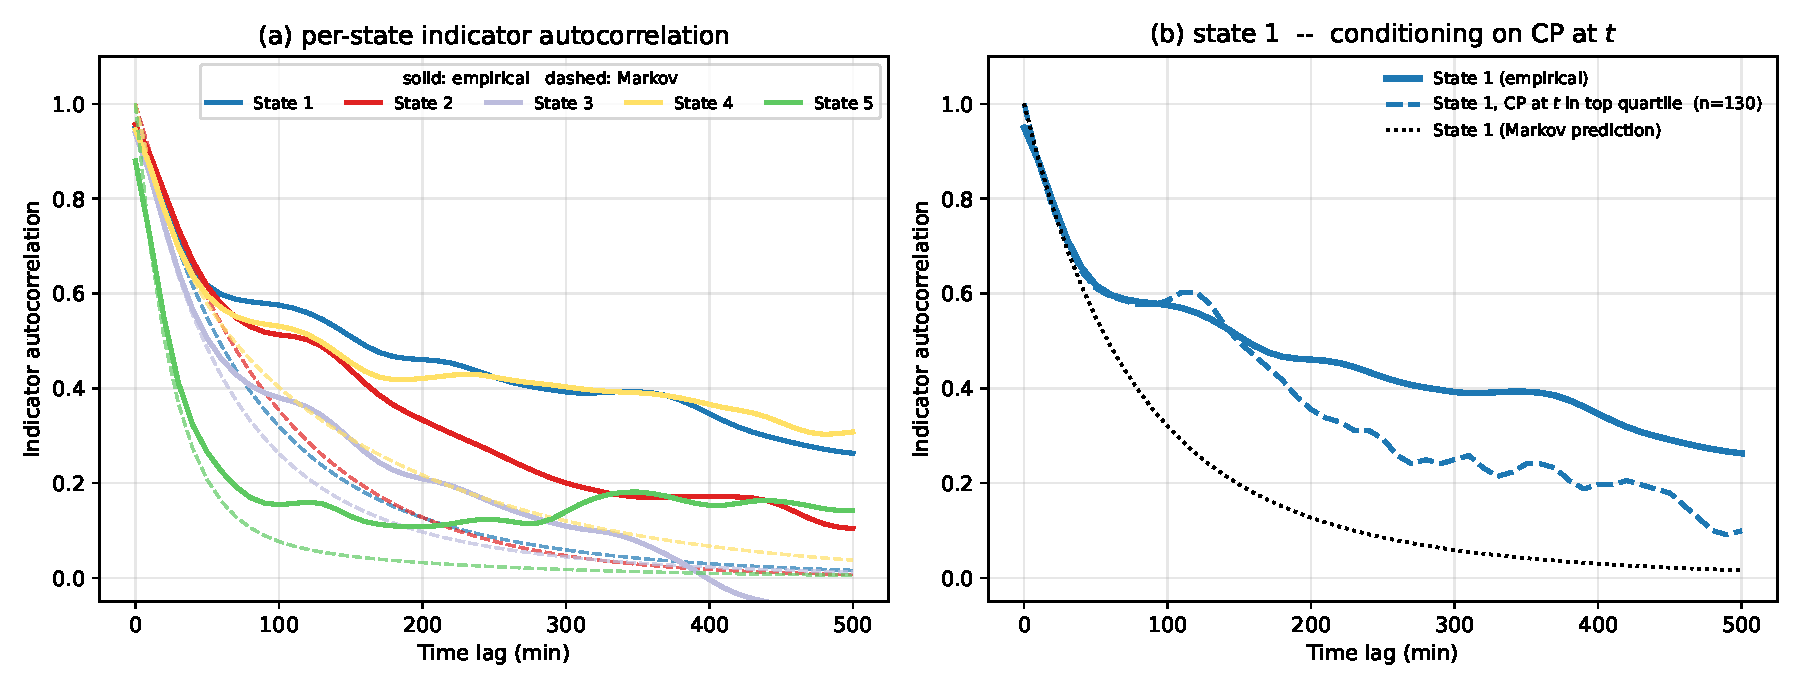
\includegraphics[width=0.9\textwidth]{fig9bis_markovianity_coldpools.pdf}
    \caption{\textbf{Markovianity assessment.} \textbf{(a)}~Per-state indicator autocorrelations (solid) and their Markov predictions (dashed, same colour); states~1 and~4 sit visibly above their predictions, the others track theirs closely. \textbf{(b)}~State-1 autocorrelation: empirical (solid blue), Markov prediction (dotted black), and empirical conditioned on $\mathrm{CP}(t)>\mathrm{CP}_\star$ at the starting time (dashed blue), which closes $\sim$30\% of the empirical--Markov gap at a 200~min lag.}
    \label{fig:autocorrelation}
\end{figure*}

\section{Discussion}

Convection varies widely even under a fixed forcing, yet this variability is structured, not random. We represented the flow with isentropic analysis and encoded it into a low-dimensional latent space, where its evolution reduces to a Markov chain over a few discrete states. Five states proved enough to recover physically meaningful convective regimes and to follow the trajectories convection takes between them. This chain is nearly memoryless, with a single slow eigenmode ($\lambda_2\approx0.94$, $\tau_2\approx172$~min) that alternates two regimes, organized and unorganized, around a dominant suppressed background ($\pi_3=37\%$); two competing routes emerge, a direct ascent into deep convection and a slower drift through weakly organized phases. The framework's distinctive feature is that departures from Markovianity \emph{diagnose} what the discrete partition omits: states~1 and~4 persist beyond their Markov prediction, and conditioning on cold-pool intensity closes $\sim$30\% of that gap at a $200$~min lag, identifying cold pools as one measurable carrier of the hidden memory.

These results describe a single, idealized forcing---fixed vertical shear in radiative--convective equilibrium---and the simplicity of the latent space may partly reflect that control: a more variable or transient forcing could populate a higher-dimensional space with more states and stronger non-Markovianity. Testing this is the natural next step. Because the transition matrix is a function of the forcing, repeating the construction across shear regimes---weak (popcorn), moderate, strong (supercritical squall lines)---turns convective organization into a measurable dynamical observable: under stronger shear the organized-state persistence $T_{ii}$ and eigenmode time scales should lengthen, and the direct route into deep convection should dominate. Sharper internal descriptors---cold-pool age, gust-front strength, mesoscale moisture, or cluster geometry---should each close more of the memory gap, every increment naming another slow variable a memory-aware parameterization must track.

\section*{Data and Code Availability}

The idealized squall-line SAM simulations (27 days at 2-minute resolution, with 1D, 2D, and 3D outputs) are available via Globus (link to be provided). All code is openly available at \url{https://github.com/sososquirrel/troposwhere}, including the model implementation and the scripts to reproduce all figures. Full methods---simulation setup, isentropic preprocessing, model architecture, training, and sensitivity tests---are given in the Supplemental Material.

\section*{Acknowledgments}

We are grateful to Juan Nathanael and Carla Roesch for discussions on Koopman operators, and to Fabrizio Falasca and Matthieu Blanke for recommendations on the dynamical systems literature. We also thank Sara Shamekh, Zhe Feng, Xingchao Chen, Ruby Leung, and the WACCEM project team for valuable discussions throughout the course of this study. We thank Koichi Sakaguchi and Huancui Hu for their internal review and constructive feedback. Portions of the manuscript were rephrased with the assistance of ChatGPT (OpenAI) for language editing, and Claude (Anthropic) assisted with aspects of code development and cleaning; all scientific ideas, analysis, and conclusions were developed by the authors. This research was supported by the Office of Science of the U.S. Department of Energy (DOE), Biological and Environmental Research (BER), as part of the Regional and Global Modeling and Analysis program area under the Water Cycle and Climate Extremes Modeling (WACCEM) project. S.A. designed the research, performed the simulations, developed the methods and code, and wrote the manuscript. O.P. contributed to the methodological development and the code and participated in the analysis and discussions. P.G. contributed to the interpretation of the results and to writing the manuscript.

\bibliographystyle{apsrev4-2}
\bibliography{biblio}

\end{document}
